% =====================================================================
%  English translation — regenerated paragraph by paragraph from
%    中: 基于生成式安全约束与闭环修正的扩散模型轨迹规划方法
%        （2026-10-23 19:38 版源稿 + 集合记号修正）
%    中: §4 实验与结果分析（同源稿第 218–300 行）
%
%  Sections I–III: source paragraphs 1–45 (strict 1:1)
%  Section IV    : source §4.1–§4.5 — 14 paragraphs + 3 tables
%                  (supplied figures restored with in-text references)
%  Layout: IEEE Robotics and Automation Letters (IEEEtran, journal)
%  Supplied method and experiment figures inserted; CARLA examples combined into one figure.
%
%  Compile:  pdflatex main.tex  (twice; no BibTeX, the source has no refs)
% =====================================================================
\documentclass[journal]{IEEEtran}

\usepackage{amsmath}
\usepackage{amssymb}
\usepackage{amsfonts}
\usepackage{url}
\usepackage[hidelinks]{hyperref}
\usepackage{bm}
\usepackage{graphicx}
\usepackage{dblfloatfix}
\usepackage[nospread]{flushend}
\graphicspath{{figures/prepared/}}

% Compact IEEE two-column floats; retain the class fonts and page geometry.
\setlength{\textfloatsep}{8pt plus 2pt minus 2pt}
\setlength{\dbltextfloatsep}{8pt plus 2pt minus 2pt}
\setlength{\floatsep}{6pt plus 2pt minus 1pt}
\setlength{\dblfloatsep}{7pt plus 2pt minus 1pt}
\setlength{\abovecaptionskip}{4pt}
\setlength{\belowcaptionskip}{0pt}
\renewcommand{\topfraction}{0.93}
\renewcommand{\bottomfraction}{0.88}
\renewcommand{\dbltopfraction}{0.93}
\renewcommand{\textfraction}{0.07}
\renewcommand{\floatpagefraction}{0.85}
\renewcommand{\dblfloatpagefraction}{0.85}
\setcounter{topnumber}{4}
\setcounter{bottomnumber}{3}
\setcounter{totalnumber}{7}
\setcounter{dbltopnumber}{3}

\newcommand{\R}{\mathbb{R}}
\newcommand{\ctrl}{H_{\mathrm{ctrl}}}
\newcommand{\ctrlf}{\widetilde{H}_{\mathrm{ctrl}}}
\newcommand{\hell}{H_{\mathrm{ell}}}
\newcommand{\Qraw}{\widehat{Q}_{0,\mathrm{raw}}^{(t)}}
\newcommand{\Qbdry}{\widehat{Q}_{0,\mathrm{bdry}}^{(t)}}
\newcommand{\Qalm}{Q_{0,\mathrm{ALM}}^{(t)}}
\newcommand{\abar}{\bar{\alpha}}

\begin{document}

\title{Diffusion-Based Trajectory Planning with Generative Safety
Constraints and Closed-Loop Correction}

\author{Author~Name,~\IEEEmembership{Member,~IEEE,}
        Author~Name,~\IEEEmembership{Member,~IEEE,}
        and~Author~Name,~\IEEEmembership{Senior~Member,~IEEE}%
\thanks{Manuscript received XXXX; revised XXXX.}}

\markboth{IEEE ROBOTICS AND AUTOMATION LETTERS. PREPRINT VERSION}%
{Author \MakeLowercase{\textit{et al.}}: Diffusion-Based Trajectory
Planning with Generative Safety Constraints and Closed-Loop Correction}

\maketitle

% ---------- 源稿段 1：摘要 ----------
\begin{abstract}
Diffusion models offer a data-driven and multimodal way of generating
trajectories, yet the generation process itself cannot explicitly guarantee
trajectory safety. Existing safety-guided approaches focus mainly on guiding
and correcting a trajectory under a given constraint set, whereas work that
generates safety constraints from the environment structure and the planning
task, and then uses the resulting safety features to guide diffusion
denoising, remains limited. This paper proposes a diffusion-based trajectory
planning method with generative safety constraints and closed-loop
correction. Combining the environmental topology with local obstacle
information, the method generates a task-relevant convex safe corridor
through local ellipse prediction and convex region construction, and extracts
local safety features that guide diffusion denoising, while the convex safe
corridor supplies explicit safety constraints for trajectory correction.
During reverse diffusion, an augmented Lagrangian method corrects the
predicted control points, and the corrected result is used both for the
sampling state update and as historical feature feedback, forming a
closed-loop safety correction mechanism. Experiments on road scenes built in
CARLA show that, under identical test conditions, all compared methods
produce trajectory collisions to varying degrees, whereas the proposed method
exhibits no collision among any of the test trajectories, indicating superior
safety performance.
\end{abstract}

% ---------- 源稿段 2：关键词 ----------
\begin{IEEEkeywords}
Diffusion-based trajectory planning, generative safety constraints, convex
safe corridor, closed-loop safety correction, augmented Lagrangian method.
\end{IEEEkeywords}

\section{Introduction}
% ---------- 源稿段 3 ----------
\IEEEPARstart{B}{y} learning the probability distribution of trajectory data,
diffusion models provide a data-driven and multimodal means of trajectory
planning. They have already been applied to task-conditioned trajectory
generation and optimization: Diffuser generates goal-directed trajectories
under cost guidance, whereas MPD combines a learned trajectory prior with cost
gradients. Learning a trajectory distribution, however, does not by itself
ensure that the generated result satisfies the safety constraints of the
environment. In non-convex environments with complex obstacle layouts and
several feasible routes, a generated trajectory may depart from obstacle-free
space and thus incur a collision risk. Preserving the multimodal generative
capability of diffusion models while improving trajectory safety is therefore
a central problem for diffusion-based trajectory planning.

% ---------- 源稿段 4 ----------
To improve safety, previous work has introduced explicit safety constraints
into the reverse diffusion process. SafeDiffuser, for instance, constrains
trajectory generation with control barrier functions (CBFs), and Projected
Diffusion Models correct infeasible predictions through projection-based
optimization. Such methods concentrate on how a given safety constraint is
used to guide or correct the generated trajectory; the constraint is usually a
predefined function or feasible set rather than one obtained by learning the
spatial structure of the environment. Moreover, the safety constraint acts on
the sampling process mainly through gradient guidance or optimization-based
correction, and the direct exploitation of local safety features inside the
denoising network has received comparatively little attention. How to generate
task-relevant safety constraints from the environmental topology and local
obstacle information, how to have the local safety features learned during
generation participate in diffusion denoising, and how to exploit the generated
constraints for continuous-trajectory correction are therefore the primary
questions addressed in this paper.

% ---------- 源稿段 5 ----------
Beyond the generation and application of safety constraints, the way
historical correction information is exploited across the multi-step reverse
diffusion process also warrants attention. Existing constraint-guided and
optimization-based methods can correct the current predicted trajectory and
influence subsequent generation through the sampling state update, but the
earlier correction is not necessarily supplied to the denoising network as an
explicit condition. Subsequent predictions may therefore repeat similar
constraint violations and require the safety correction to be executed again.
How to incorporate historical safety corrections into the conditioning
representation of the denoising network, so that they affect not only the
sampling state update but also subsequent trajectory prediction, is the second
question addressed here.

% ---------- 源稿段 6 ----------
To address these questions, this paper proposes TrajSafe-Diffuser, a
diffusion-based trajectory planning method with generative safety constraints
and closed-loop correction. For the construction of generative safety
constraints, feasible routes are selected from the free space of the
environment according to the planning task, local ellipse parameters are
predicted along the selected route, and a task-relevant convex safe corridor is
obtained by convex region construction. Unlike approaches that merely use a
given constraint to guide or correct a trajectory, local safety features are
learned together with the safety constraints and serve as conditioning
information for the denoising network, while the generated convex safe corridor
establishes explicit safety constraints, so that environment- and task-related
safety information acts separately on trajectory prediction and on constraint
correction.

% ---------- 源稿段 7 ----------
For closed-loop safety correction, the generated convex safe corridor
constrains the trajectory predicted by reverse diffusion, and an augmented
Lagrangian method corrects the predicted control points. Rather than using the
corrected result only for the sampling state update, a historical safety
feedback mechanism is designed that injects the corrected control points and
their change into the subsequent denoising network in a gated manner, so that
the denoising prediction can exploit earlier safety corrections and a closed
loop is formed between trajectory generation and safety correction.

% ---------- 源稿段 8-11：贡献 ----------
The main contributions of this paper are as follows.
\begin{enumerate}
% 段 9
\item \emph{A diffusion-based trajectory planning framework with generative
safety constraints and closed-loop correction.} Aiming at safe trajectory
generation in complex non-convex environments, it combines task-relevant safety
constraint generation with diffusion-based trajectory planning, yielding a
framework that integrates safety-conditioned guidance, explicit constrained
optimization and historical feedback.

% 段 10
\item \emph{A generative safety constraint construction method for complex
non-convex environments.} Candidate routes are matched against the
environmental topology and the planning task; local ellipse parameter
prediction together with convex region construction produces a task-relevant
convex safe corridor, and local safety features are learned simultaneously, so
that the generated safety information can be used separately for diffusion
denoising guidance and for continuous-trajectory constraint correction.

% 段 11
\item \emph{A closed-loop safety correction mechanism based on constrained
optimization and historical feedback.} The augmented Lagrangian method corrects
the predicted control points during reverse diffusion and the result updates
the subsequent sampling state, while a gating mechanism injects the historical
correction into the denoising network so that earlier safety corrections
participate in later trajectory prediction.
\end{enumerate}

\section{Problem Definition}
% ---------- 源稿段 12 ----------
Consider trajectory planning in a two-dimensional static environment. Given an
occupancy grid map $O\in\{0,1\}^{H\times W}$, a start $\bm S\in\R^2$ and a
goal $\bm G\in\R^2$, the objective is to generate a continuous trajectory that
connects the start and the goal while satisfying the obstacle-avoidance
requirement of the environment.

% ---------- 源稿段 13 ----------
The trajectory is represented by a clamped cubic B-spline defined by
$C=48$ control points. Denoting the control point set by
$Q=[q_0,\ldots,q_{C-1}]\in\R^{C\times2}$, the continuous trajectory is
\begin{equation}
\tau_Q(u)=\sum_{j=0}^{C-1}B_{j,3}(u)\,q_j,\qquad u\in[0,1],
\end{equation}
where $B_{j,3}$ is the cubic B-spline basis function and $u$ the curve
parameter. Owing to the endpoint interpolation property of clamped B-splines,
$q_0=\bm S$ and $q_{C-1}=\bm G$ are fixed and diffusion sampling is performed
only on the interior control points.

% ---------- 源稿段 14 ----------
Let $\mathcal F(O)$ denote the obstacle-free space of the map. The trajectory
is then required to satisfy
\begin{equation}
q_0=\bm S,\quad q_{C-1}=\bm G,\quad
\tau_Q(u)\in\mathcal F(O),\quad \forall u\in[0,1].
\end{equation}
A conditional diffusion model is used to learn the control point distribution
$p_\theta(Q\mid O,\bm S,\bm G)$ and thereby generate different candidate
trajectories. Since probabilistic modeling cannot directly guarantee the
continuous obstacle-avoidance condition above, this paper further studies how
to generate safety constraints from the environment structure and the planning
task, and how to improve the safety feasibility of the generated trajectory
through constraint correction and historical feedback during reverse diffusion.

\section{Method}
% ---------- 源稿段 15（原稿方法引言只有这一段） ----------
The overall structure of TrajSafe-Diffuser, shown in Fig.~\ref{fig:framework}, comprises three modules: feature
encoding and fusion, generative safety constraint construction, and trajectory
denoising with closed-loop correction. The model first encodes the environment,
the current noisy control points and the historical feedback into conditioning
features used for route matching and trajectory prediction. Candidate route
matching, local ellipse prediction and convex region construction then generate
the safety constraints, and local safety features are extracted to guide
denoising. Finally, the reverse-diffusion prediction, after explicit constraint
correction, takes part in subsequent generation through the sampling state
update and the historical feedback.


\begin{figure*}[!tb]
\centering
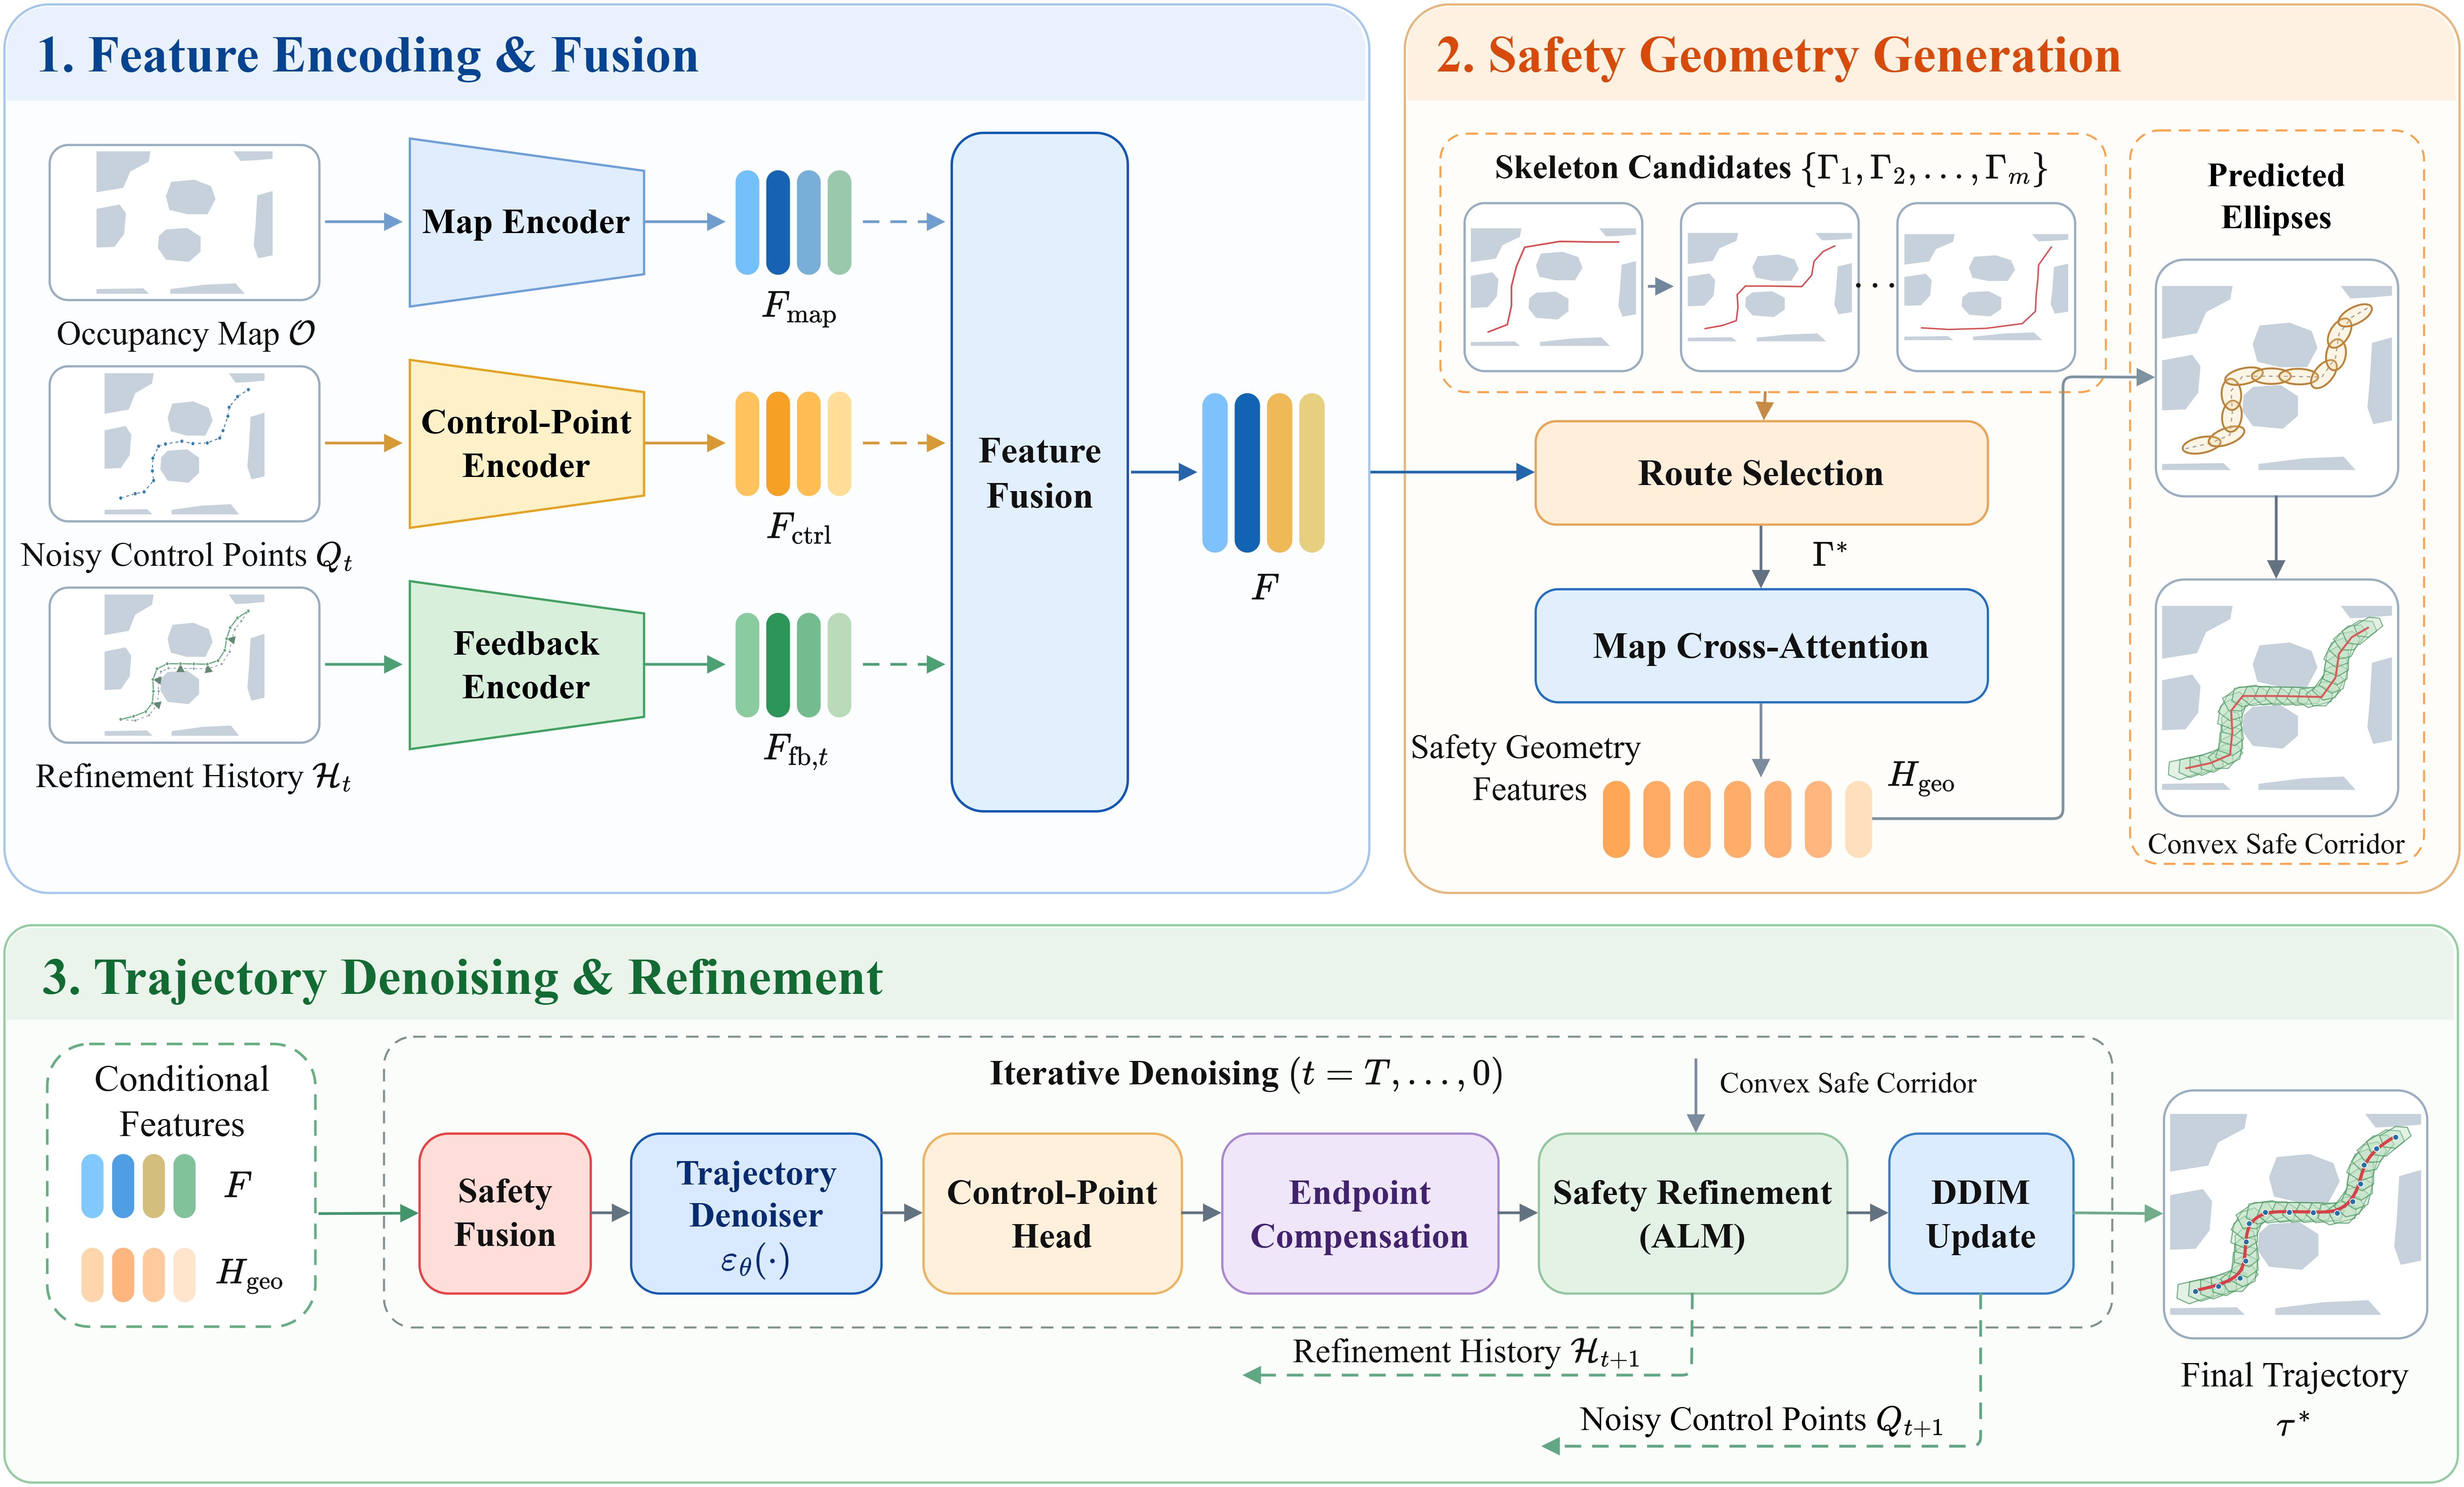
\includegraphics[width=\textwidth]{fig01_framework.png}
\caption{Overall framework of TrajSafe-Diffuser. Feature encoding and fusion condition safety geometry generation and trajectory denoising. ALM correction updates the sampling state and supplies historical safety feedback.}
\label{fig:framework}
\end{figure*}

\subsection{Feature Encoding and Fusion}

\subsubsection{Map and Control Point Feature Encoding}
% ---------- 源稿段 16 ----------
A multi-scale convolutional encoder--decoder network is used to extract
occupancy map features. The encoder captures global environment information
through successive downsampling, while the decoder preserves local spatial
information through upsampling and fusion of intermediate-layer features. After
channel mapping and positional encoding, a global map feature
$C_G\in\R^{256\times128}$ and a local map feature
$C_E\in\R^{1024\times128}$ are obtained, corresponding to spatial resolutions
of $16\times16$ and $32\times32$. $C_G$ is used for control point feature
encoding and conditional denoising, whereas $C_E$ is used for local safety
feature extraction.

% ---------- 源稿段 17 ----------
For the current noisy control points $Q_t$, the coordinates are first
positionally encoded and mapped by an MLP, and a control point index encoding
is then added, giving the initial control features
\begin{equation}
X_j^{(0)}=\operatorname{MLP}_{T}\!\left(\Phi_{xy}(q_{t,j})\right)
+\operatorname{PE}_{1D}(j).
\end{equation}

% ---------- 源稿段 18 ----------
Eight conditional attention blocks are then applied to extract the relations
among control points and the environment information. Each block contains
control point self-attention, global-map cross-attention and a feed-forward
network, and the diffusion time condition is introduced through adaptive layer
normalization. Four attention heads and 128-dimensional features are used,
finally yielding the control features $\ctrl\in\R^{48\times128}$.

\subsubsection{Historical Safety Feedback Fusion}
% ---------- 源稿段 19 ----------
To make use of earlier safety corrections, the most recent corrected control
points that passed the constraint check, $Q_{\mathrm{hist}}$, the corresponding
correction $\Delta Q_{\mathrm{hist}}$ and a validity flag $v\in\{0,1\}$ are
taken as historical feedback inputs. The five-dimensional feedback vector of
each control point is encoded by an MLP into
$H_{\mathrm{fb}}\in\R^{48\times128}$.

% ---------- 源稿段 20 ----------
To regulate how strongly individual control points and feature channels exploit
the historical correction, a channel-wise gating mechanism is used:
\begin{equation}
\begin{aligned}
g&=\sigma\!\left(W_g[\ctrl;H_{\mathrm{fb}}]+b_g\right),\\
\ctrlf&=\ctrl+v\,g\odot H_{\mathrm{fb}},
\end{aligned}
\end{equation}

% ---------- 源稿段 21 ----------
where $[\cdot;\cdot]$ denotes feature concatenation, $\sigma$ the sigmoid
function and $\odot$ the element-wise product, with
$g\in\R^{48\times128}$. When $v=0$ the historical feedback takes no part in the
fusion; otherwise the gating weights adapt, according to the current control
features and the historical feedback, the correction applied to each control
point and feature channel. The fused features $\ctrlf$ are used both for
candidate route matching and for conditional denoising, so that the historical
correction participates in the subsequent route selection and trajectory
prediction.

\subsection{Generative Safety Constraint Construction}

\begin{figure*}[!tb]
\centering
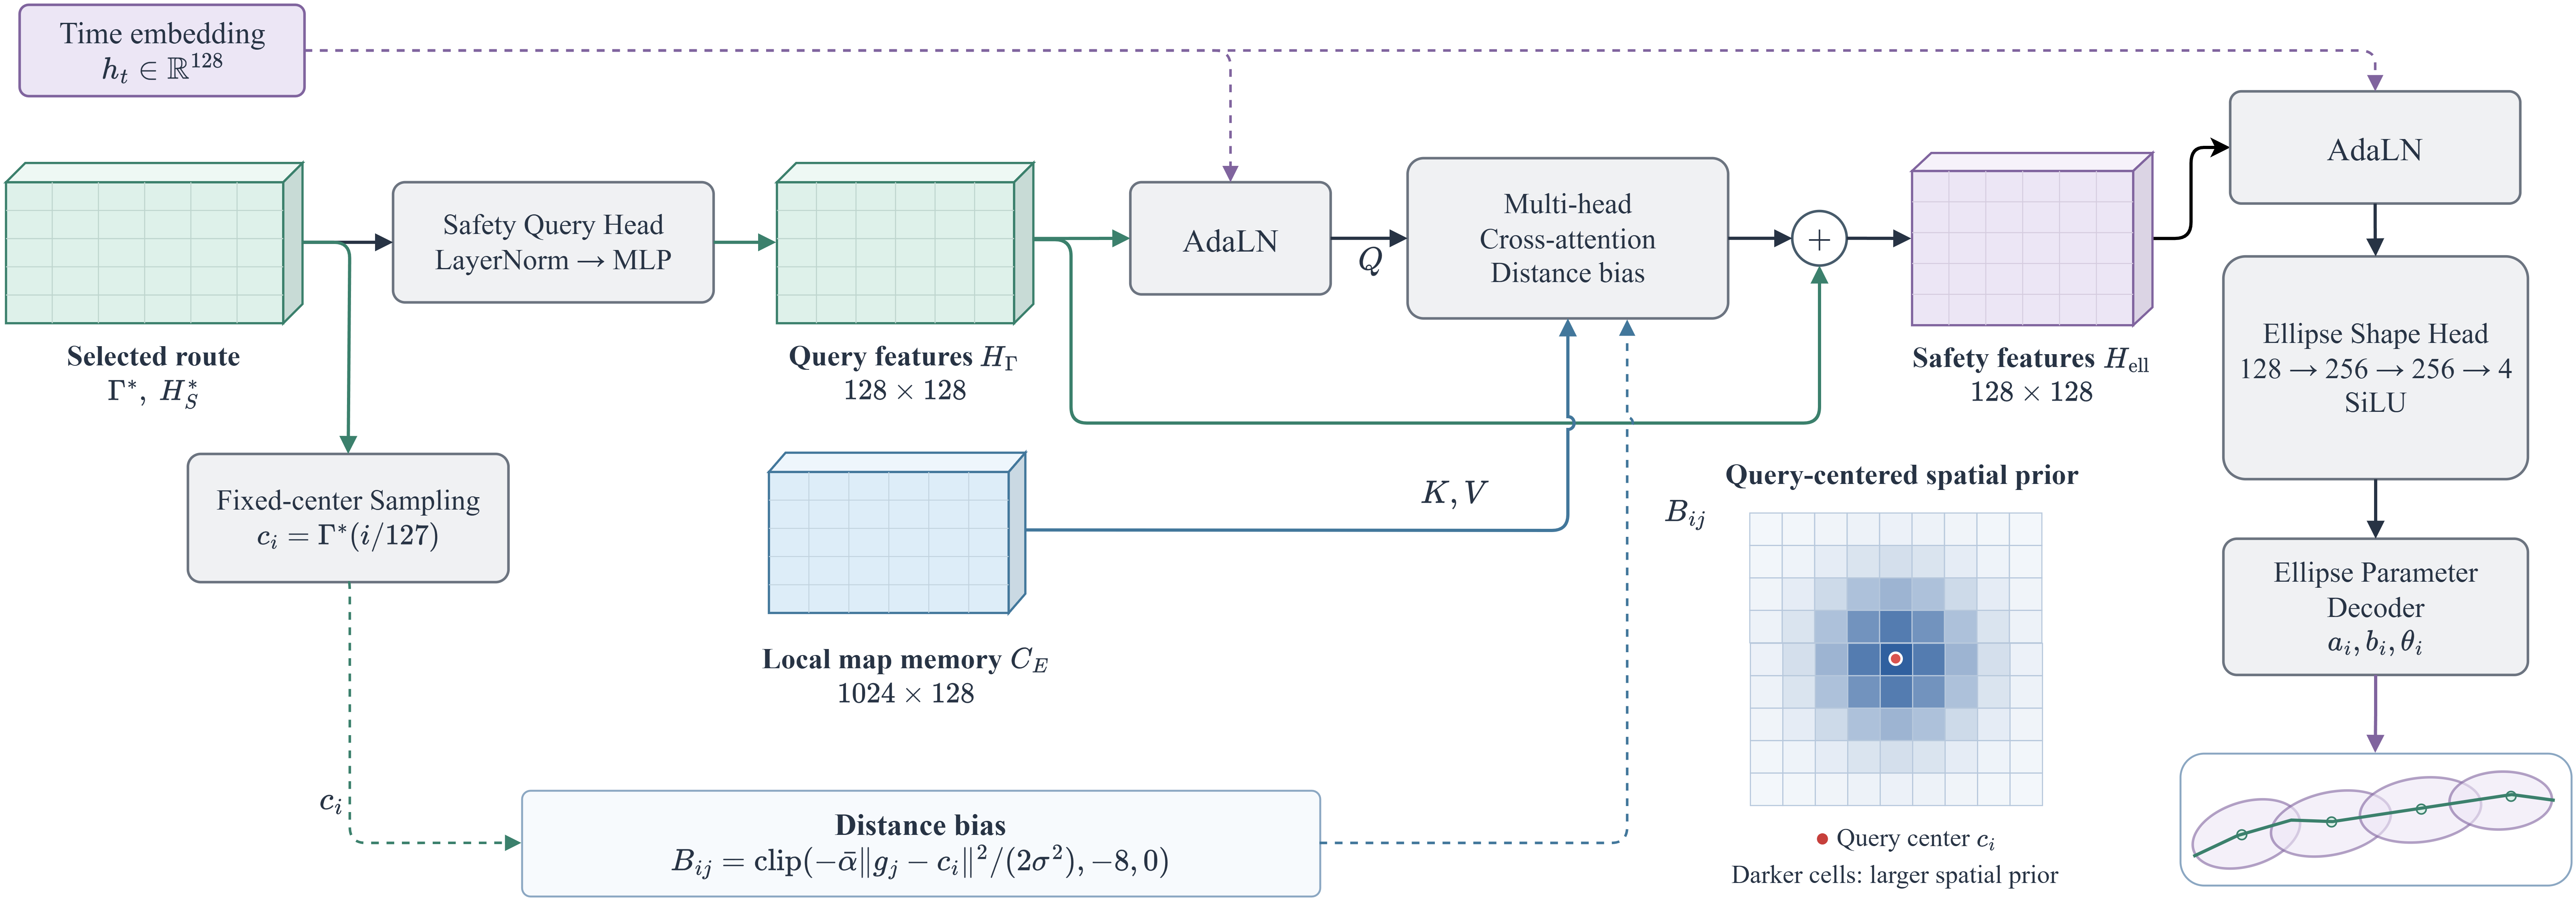
\includegraphics[width=\textwidth]{fig02_safety_generation.png}
\caption{Local safety feature extraction and ellipse prediction. Selected-route features query local map features through time-conditioned cross-attention with a spatial distance bias. The predicted ellipses initialize the subsequent convex-region construction.}
\label{fig:safety}
\end{figure*}



\subsubsection{Candidate Skeleton Route Matching and Selection}
% ---------- 源稿段 22 ----------
First, the Guo--Hall thinning algorithm is applied to the occupancy map to
extract the free-space skeleton and to build a skeleton graph, on which up to
$M$ candidate routes $\{\Gamma_m\}_{m=1}^{M}$ connecting the start $\bm S$ and
the goal $\bm G$ are searched. Different skeleton routes represent different
ways of circumventing the obstacles, so that the model retains several planning
options at the topological level instead of presupposing a single route; the
diffusion model then generates a continuous trajectory under the safety
constraints associated with the selected route.

% ---------- 源稿段 23 ----------
Each candidate route is resampled at equal arc length into 128 points; the
two-dimensional coordinates of the sample points are positionally encoded and
mapped by an MLP, and sequence positional encoding together with self-attention
is used to extract the route features $H_{S,m}\in\R^{128\times128}$. With the
fused control features $\ctrlf$ of Section~III-A as queries and the candidate
route features as keys and values, time-conditioned cross-attention computes
the matching features. Average pooling along the control point dimension
followed by a scoring network and a masked softmax gives the route selection
probabilities $\pi_m$, and the route $\Gamma^*$ with the highest probability is
selected.

\subsubsection{Local Safety Feature Extraction and Convex Safe Corridor Generation}
% ---------- 源稿段 24 ----------
As illustrated in Fig.~\ref{fig:safety}, with the features $H_{S,*}$ of the selected route $\Gamma^*$ as queries and the
local map features $C_E$ as keys and values, time-conditioned cross-attention
extracts the local obstacle information. To strengthen attention to the spatial
structure around the skeleton sample points, a distance bias is introduced into
the attention scores:
\begin{equation}
\mathcal B_{ij}^{\mathrm{geo}}
=\operatorname{clip}\!\left(
-\frac{\abar_t\,\lVert c_i-z_j\rVert_2^2}
{2\sigma_{\mathrm{geo}}^2},
-b_{\mathrm{clip}},0\right),
\end{equation}
\begin{equation}
\operatorname{Attn}(Q_a,K_a,V_a)
=\operatorname{Softmax}\!\left(
\frac{Q_aK_a^{\mathsf T}}{\sqrt{d_k}}+\mathcal B^{\mathrm{geo}}
\right)V_a,
\end{equation}

% ---------- 源稿段 25 ----------
where $c_i$ is the coordinate of the $i$-th sample point of the selected
skeleton route and $z_j$ the spatial position corresponding to local map
feature $j$. The distance bias reduces the attention weight of map features
that are far from the skeleton sample points. Residual fusion of the
cross-attention output with the query features yields the local safety features
$\hell\in\R^{128\times128}$, from which an ellipse prediction head then outputs
the local ellipse parameters.

% ---------- 源稿段 26 ----------
To ensure that the convex safety region construction starts from a valid
free-space position, the free-space-checked skeleton sample points $c_i$ are
used as ellipse centers, which avoids the problem that predicting the centers
directly may place them inside obstacles. The network predicts only the scale
and orientation of the ellipse:
\begin{equation}
e_i=(\log a_i,\ \log b_i,\ \cos 2\theta_i,\ \sin 2\theta_i),
\end{equation}

% ---------- 源稿段 27 ----------
where $a_i$, $b_i$ and $\theta_i$ denote the semi-axis lengths and the rotation
angle of the ellipse. The predicted ellipse serves as a local geometric prior
and does not by itself guarantee obstacle-free space. Taking the skeleton
centers in free space and the predicted ellipses as a basis, a deterministic
convex region construction is further performed according to the obstacle grid,
the map boundary and a safety margin, giving
\begin{equation}
\mathcal R_i=\{x\in\R^2\mid A_ix\leq b_i\}.
\end{equation}

% ---------- 源稿段 28 ----------
The local convex regions are arranged in order along the selected skeleton
route. Where adjacent regions overlap insufficiently, an intermediate position
between the corresponding skeleton sample points along the route is taken as a
seed, and an additional obstacle-free convex region is constructed for bridging,
forming a continuous convex safe corridor $\mathcal C$. Finally, the local
safety features $\hell$ are used to guide diffusion denoising, while the convex
safe corridor $\mathcal C$ provides explicit safety constraints for the
continuous trajectory.

\subsection{Trajectory Denoising and Closed-Loop Safety Correction}

\subsubsection{Safety-Conditioned Denoising}
% ---------- 源稿段 29 ----------
With the fused control features $\ctrlf$ as queries and the local safety
features $\hell$ as keys and values, multi-head cross-attention extracts the
safety information corresponding to each control point, and residual fusion
followed by an MLP mapping gives the safety-conditioned features
$F\in\R^{48\times128}$. $F$ is then fed to three conditional denoising blocks
that predict the clean control points $\Qraw$, conditioned on the global map
features $C_G$ and the diffusion time step $t$. Each block contains control
point self-attention, map cross-attention and a feed-forward network.

% ---------- 源稿段 30 ----------
Finally, endpoint correction is applied to the predicted control points,
yielding the control points $\Qbdry$ that satisfy the start and goal
constraints.

\subsubsection{Continuous-Trajectory Safety Constraint and ALM Correction}

\begin{figure*}[!tb]
\centering
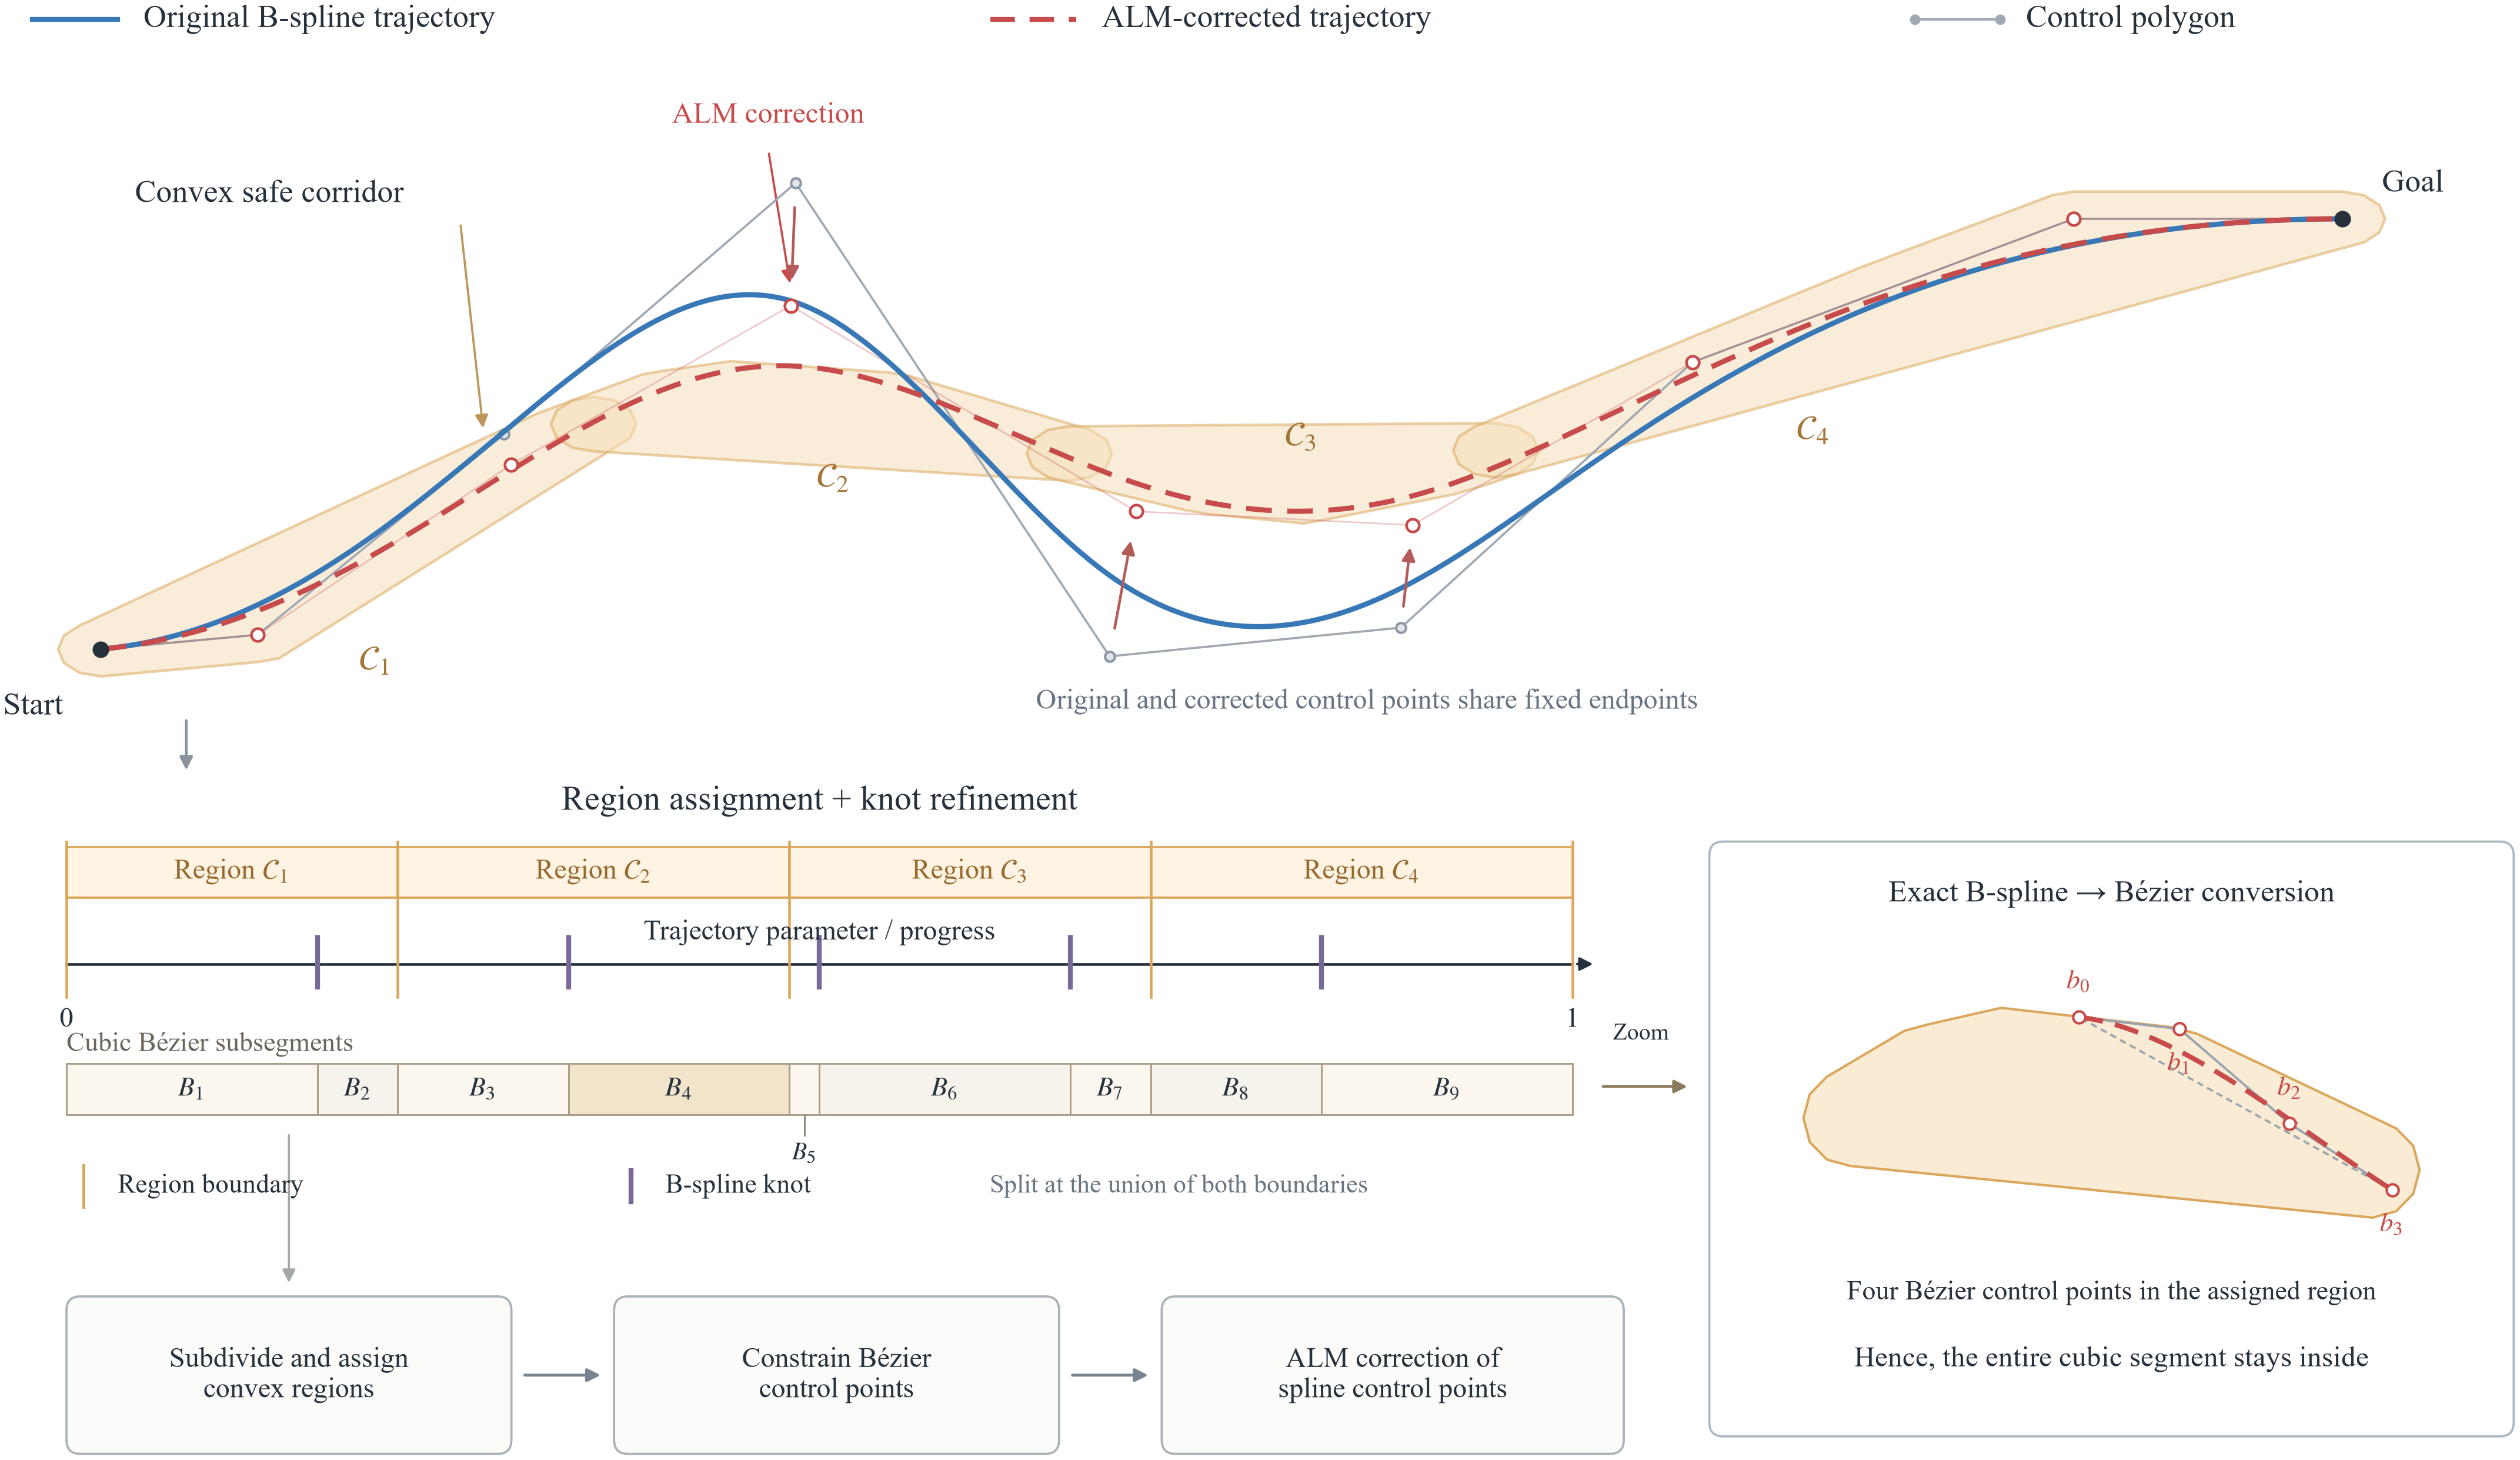
\includegraphics[width=0.8\textwidth]{fig03_alm.png}
\caption{Continuous-trajectory safety constraints and ALM correction. Region responsibility boundaries and B-spline knots define cubic B\'ezier subsegments. Constraining their four control points to the assigned convex region gives continuous segment containment; ALM adjusts the spline control points while fixing the endpoints.}
\label{fig:alm}
\end{figure*}


% ---------- 源稿段 31 ----------
The diffusion model outputs a cubic B-spline curve defined by $C=48$ control
points, whereas the safe corridor consists of several local convex regions
arranged along the skeleton route. Constraining the original B-spline control
points directly inside the local convex regions easily produces conservative
constraints, because the convex hull of the control points need not match the
extent of a region. The B-spline is therefore subdivided and converted exactly
into cubic B\'ezier subsegments, so that the safety constraint acts on a
shorter continuous curve segment.

% ---------- 源稿段 32 ----------
Let the safe corridor contain $N$ convex regions ordered by route progress, the
$i$-th region corresponding to a normalized progress $s_i\in[0,1]$. To make
explicit the curve range constrained by each region, the parameter intervals
are delimited by the progress midpoints of adjacent regions:
\begin{equation}
\begin{aligned}
m_i&=\frac{s_i+s_{i+1}}{2},\quad i=1,\ldots,N-1,\\
m_0&=0,\quad m_N=1.
\end{aligned}
\end{equation}

% ---------- 源稿段 33 ----------
The B-spline parameter interval $[m_{i-1},m_i]$ is assigned to the $i$-th
convex region. Since a cubic B-spline corresponds to a single cubic polynomial
only within a knot interval, a curve crossing a knot cannot be represented
exactly by one cubic B\'ezier curve. The region boundaries are therefore merged
with the interior knots of the B-spline, sorted and de-duplicated, giving $K$
subsegments $[u_{k-1},u_k]$. Each subsegment inherits the constraint of its
region and does not cross a B-spline knot. This partition only specifies the
correspondence between regions and curve parameters; the trajectory is not
required to already lie inside the corresponding region before correction.

% ---------- 源稿段 34 ----------
Let $Q\in\R^{C\times2}$ be the control point matrix of the original B-spline,
$\mathbf n(u)\in\R^{1\times C}$ the row vector of basis functions, and
$h_k=u_k-u_{k-1}$ the subsegment length. The four B\'ezier control points of
subsegment $k$ satisfy $\bm\beta_k=E_kQ$, where the conversion matrix is
\begin{equation}
E_k=
\begin{bmatrix}
\mathbf n(u_{k-1})\\[2pt]
\mathbf n(u_{k-1})+\tfrac{h_k}{3}\mathbf n'(u_{k-1})\\[3pt]
\mathbf n(u_k)-\tfrac{h_k}{3}\mathbf n'(u_k)\\[3pt]
\mathbf n(u_k)
\end{bmatrix},
\end{equation}

% ---------- 源稿段 35 ----------
where $\mathbf n'(u)$ is the derivative of the basis functions, evaluated
one-sidedly at a knot according to the subsegment in question. This conversion
does not change the curve shape and introduces no additional optimization
variable.

% ---------- 源稿段 36 ----------
Owing to the convex-hull property of B\'ezier curves, if the four control
points of a subsegment all lie inside the corresponding convex safe region
$\mathcal R_k=\{x\in\R^2\mid A_kx\leq b_k\}$, the whole curve segment lies
inside that region. The continuous safety condition can therefore be written as
\begin{equation}
A_k\bm\beta_{k,j}\leq b_k,\qquad j=1,2,3,4.
\end{equation}

% ---------- 源稿段 37 ----------
Substituting $\bm\beta_k=E_kQ$ and collecting the subsegments gives linear
inequalities $g(Q)\leq0$ in $Q$. Given that every convex region has been
verified obstacle-free, satisfying these constraints guarantees that the whole
continuous trajectory lies inside the safety region, and not merely that a
finite set of sample points is collision-free. This is a sufficient condition
for continuous safety, but it does not guarantee that the optimization problem
is feasible.

% ---------- 源稿段 38 ----------
As shown in Fig.~\ref{fig:alm}, the augmented Lagrangian method (ALM) is used to apply safety correction to the
B-spline control points, satisfying the continuous-trajectory safety constraint
while preserving the shape of the original predicted trajectory as far as
possible. Taking the endpoint-corrected control points
$Q^{\mathrm{ref}}=\Qbdry$ as reference and defining the control point correction
$\Delta Q=Q-Q^{\mathrm{ref}}$, the following constrained optimization problem is
established:
\begin{equation}
\begin{aligned}
\min_{Q}\quad
&\frac{\lambda_p}{2}\lVert\mathbf B\Delta Q\rVert_F^2
+\frac{\lambda_s}{2}\lVert D_2\mathbf B\Delta Q\rVert_F^2\\
\mathrm{s.t.}\quad
&g(Q)\leq0,\\
&q_0=\bm S,\qquad q_{C-1}=\bm G,
\end{aligned}
\end{equation}

% ---------- 源稿段 39 ----------
where $\mathbf B$ is the B-spline sampling basis matrix, $\mathbf B\Delta Q$ the
trajectory correction displacement, and $D_2$ the second-difference matrix. The
two objective terms limit, respectively, the offset of the trajectory from the
original prediction and the local fluctuation of the correction displacement
along the trajectory. By introducing constraint multipliers and penalty terms,
the ALM iteratively adjusts the interior control points in order to reduce the
safety constraint violation while keeping the start and goal fixed, finally
yielding the corrected control points $\Qalm$.

\subsubsection{Reverse-Diffusion Update and Historical Safety Feedback}
% ---------- 源稿段 40 ----------
To let the safety correction take part in subsequent trajectory generation, the
ALM result $\Qalm$ is taken as the clean control point estimate at the current
step, the sampling state of the next step is updated by a deterministic DDIM
update, and the start and goal are kept fixed throughout. The final sampling
step directly adopts the corrected control points.

% ---------- 源稿段 41 ----------
Meanwhile, inspired by the idea of self-conditioning, the safety correction
result of the previous reverse-diffusion step is used as an auxiliary condition
for the subsequent network prediction. The historical feedback comprises the
corrected control points, the correction relative to the original prediction and
a validity flag:
\begin{equation}
\begin{aligned}
Q_{\mathrm{hist}}&=\Qalm,\\
\Delta Q_{\mathrm{hist}}&=\Qalm-\Qbdry,\\
v_{\mathrm{hist}}&\in\{0,1\}.
\end{aligned}
\end{equation}

% ---------- 源稿段 42 ----------
This information takes part in the trajectory prediction of the next
reverse-diffusion step through the gated fusion module of Section~III-A. Unlike
self-conditioning, which feeds the network prediction back directly, this
mechanism further introduces the control points after safety constraint
correction together with their correction, so that subsequent denoising can
exploit the historical safety correction and a closed loop is achieved between
trajectory generation and safety correction.

\subsection{Training Strategy and Loss Function}
% ---------- 源稿段 43 ----------
To enable the network to learn to exploit historical safety corrections, a
two-forward training strategy with shared parameters is adopted. First, noise is
added to the reference control points at a random diffusion time step $t$, a
first forward prediction is performed without historical feedback, and ALM
correction is applied using the offline convex safe corridor associated with the
reference route, which also constructs the historical safety feedback and the
DDIM sampling state of the next time step. The updated control points and the
historical feedback are then fed into the same network for a second forward
prediction. The two forward passes share the network parameters, and the
gradients of the second pass do not back-propagate to the first. During
training, part of the historical feedback is masked at random, so as to
accommodate the initial sampling state in which no feedback is available.

% ---------- 源稿段 44-45（按作者要求：删去表 1，改用一段文字表述） ----------
The training loss consists of three parts. The trajectory prediction losses
$\mathcal L_{\mathrm{ctrl}}$, $\mathcal L_{\mathrm{boundary}}$ and
$\mathcal L_{\mathrm{smooth}}$ supervise, respectively, control point
reconstruction, the endpoint neighbourhood and smoothness. The safety
constraint generation losses $\mathcal L_{\mathrm{topo}}$,
$\mathcal L_{\mathrm{shape}}$, $\mathcal L_{\mathrm{IoU}}$ and
$\mathcal L_{\mathrm{ell,safe}}$ supervise, respectively, route selection,
ellipse shape, region coverage and obstacle intrusion. The continuous safety
loss $\mathcal L_{\mathrm{safe}}$ penalizes continuous safety violations of the
trajectory through the B\'ezier convex-hull constraint. These losses are
combined by weighted summation to form the final training objective.

\section{Experiments and Results}

\subsection{Experimental Setup}
% ---------- 源稿 [4.1] 段 1 ----------
Experiments are conducted on a two-dimensional static occupancy grid dataset
built from CARLA road scenes. The map covers
$160\,\mathrm{m}\times160\,\mathrm{m}$ with a grid resolution of $256\times256$,
i.e., a spatial resolution of $0.625\,\mathrm{m/grid}$. The training, validation
and test sets contain 3850, 1550 and 420 samples, respectively, and the test set
is drawn from towns that did not take part in training.

% ---------- 源稿 [4.1] 段 2 ----------
Every model represents the trajectory by a cubic B-spline with 48 control points
and is trained for 200 epochs on an NVIDIA GeForce RTX 4070 with a learning rate
of $2\times10^{-4}$ and a batch size of 16. Generators D, S and A denote the base
diffusion model, the safety-conditioned model and the model trained with
historical feedback, respectively. Standard inference uses 16 DDIM steps, the
first 3 of which serve as warm-up, and the maximum number of ALM iterations is
set to 10. Unless stated otherwise, all methods are evaluated on the same 420
test samples.

% ---------- 源稿 [4.1] 段 3 ----------
The generated trajectories are evaluated in terms of safety, path quality,
geometric quality and computational efficiency. Safety is measured by the
collision rate and the mean minimum clearance, the latter being averaged over
collision-free trajectories only. Path quality is measured by the detour ratio
and the normalized root-mean-square error (NRMSE), which reflect the path-length
cost and the deviation from the reference trajectory, respectively. Geometric
quality is measured by the maximum curvature and the mean squared curvature.
Computational efficiency is measured by the mean inference time per trajectory.
Collision checking samples 512 points uniformly along the trajectory and tests
them against the occupancy grid, whereas the satisfaction of the continuous
constraint is assessed separately from the B\'ezier control-point constraints.

\subsection{Performance Comparison of Safety Planning Methods}
% ---------- 源稿 [4.2] 段 1 ----------
The proposed method is compared with unconstrained diffusion, fixed penalty
guidance, primal--dual guidance and SDF augmented Lagrangian guidance.
Unconstrained diffusion generates trajectories directly. Fixed penalty guidance
corrects a trajectory with the gradient of a collision cost defined on a signed
distance field (SDF). Primal--dual guidance alternately updates the control
variables and the constraint multipliers. SDF-ALM additionally introduces an
augmented Lagrangian penalty term. The parameters of the three SDF-based
guidance methods are all selected on the validation set.

\begin{table*}[!t]
\caption{Performance Comparison of Different Safety Planning Methods}
\label{tab:methods}
\centering
\footnotesize
\setlength{\tabcolsep}{4pt}
\begin{tabular}{lcccccc}
\hline
Method & Collision (\%) $\downarrow$ & Clearance (m) $\uparrow$ &
Detour ratio $\downarrow$ & NRMSE (\%) $\downarrow$ &
Max curvature (1/m) $\downarrow$ &
Mean sq. curvature (1/m$^2$) $\downarrow$ \\
\hline
Unconstrained diffusion & 61.19 & 2.899 & 1.0896 & 13.202 & 0.3313 & 0.00412 \\
Fixed penalty guidance  & 19.05 & 1.710 & 1.4665 & 12.066 & 1.1893 & 0.04596 \\
Primal--dual guidance   & 23.10 & 1.774 & 1.2337 & 11.904 & 0.7393 & 0.01764 \\
SDF-ALM guidance        & 23.89 & 1.763 & 1.1679 & 11.905 & 0.5872 & 0.01154 \\
\textbf{TrajSafe-Diffuser} & \textbf{0.00} & \textbf{3.255} & 1.3246 &
\textbf{8.759} & 1.0869 & 0.02182 \\
\hline
\end{tabular}
\end{table*}

% ---------- 源稿 [4.2] 段 2 ----------
Unconstrained diffusion reaches a collision rate of 61.19\%, which shows that
relying on trajectory-distribution learning alone hardly guarantees the safety of
the generated result. The three SDF-based guidance methods lower the collision
rate to 19.05\%--23.89\%, yet collisions remain. By contrast, TrajSafe-Diffuser
detects no collision among 1260 trajectories, and both its mean minimum
clearance of 3.255~m and its NRMSE of 8.759\% outperform the compared methods.

% ---------- 源稿 [4.2] 段 3 ----------
The geometric metrics exhibit a certain trade-off. The detour ratio of the
proposed method is 1.3246, higher than those of primal--dual guidance and
SDF-ALM guidance, and its mean squared curvature is also higher than that of
these two methods. Explicit safety constraints thus improve safety and
reference-tracking accuracy, but do not necessarily yield shorter or less curved
trajectories. Since the compared methods use generator D whereas the complete
method uses generator A, this experiment reflects the overall performance
difference between complete systems; the contribution of each module is analysed
in the ablation study below.

\subsection{Ablation Study and Analysis of Historical Safety Feedback}

\subsubsection{Key Module Ablation}
% ---------- 源稿 [4.3.1] 段 1 ----------
Four progressively configured variants are considered. A0 is the base diffusion
model; A1 adds the safety geometry condition; A2 further adopts feedback training
and uses the ALM correction as historical feedback but does not update the DDIM
state with the corrected result; A3 uses the corrected result simultaneously for
the historical feedback, the DDIM state update and the final output.

\begin{table}[!t]
\caption{Ablation Results of the Key Modules}
\label{tab:ablation}
\centering
\footnotesize
\setlength{\tabcolsep}{4pt}
\begin{tabular}{lcccc}
\hline
 & Collision & Clearance & Detour ratio & NRMSE \\
Configuration & (\%) $\downarrow$ & (m) $\uparrow$ &
$\downarrow$ & (\%) $\downarrow$ \\
\hline
A0: base     & 61.19 & 2.899 & 1.0896 & 13.202 \\
A1: $+$ safety cond. & 25.16 & 3.120 & 1.2278 &  7.911 \\
A2: $+$ feedback     &  3.33 & 3.225 & 1.3154 &  8.734 \\
\textbf{A3: complete} & \textbf{0.00} & \textbf{3.255} & 1.3246 &
\textbf{8.759} \\
\hline
\end{tabular}
\end{table}

% ---------- 源稿 [4.3.1] 段 2 ----------
Adding the safety geometry condition lowers the collision rate from 61.19\% to
25.16\% and the NRMSE from 13.202\% to 7.911\%. Introducing feedback training
further reduces the collision rate to 3.33\%. With A2 and A3 sharing the same
generator weights, using the ALM correction for the DDIM state update and the
final output reduces the number of collisions from 42 to 0, while the NRMSE
changes only from 8.734\% to 8.759\%. The safety geometry condition therefore
improves trajectory prediction, and feeding the safety correction directly into
the reverse diffusion process improves the final safety further. The difference
between A1 and A2 also involves a change of training strategy and should be read
as the joint effect of the feedback mechanism and its training strategy.

\subsubsection{Effect of Historical Safety Feedback on the Denoising Process}
% ---------- 源稿 [4.3.2] 段 1 ----------
To isolate the role of the historical feedback, only the historical feedback
input is switched, while the generator weights, the ALM configuration and the
safe corridor are kept identical, and the mean safety violation before ALM
correction and the mean correction magnitude over forwards 4--16 are compared.
The two groups coincide at the fourth forward; thereafter the prediction with
feedback enabled shows a lower violation and a lower correction magnitude
overall.

Figure~\ref{fig:feedback} shows the corresponding denoising-process curves.

\begin{figure}[!htb]
\centering
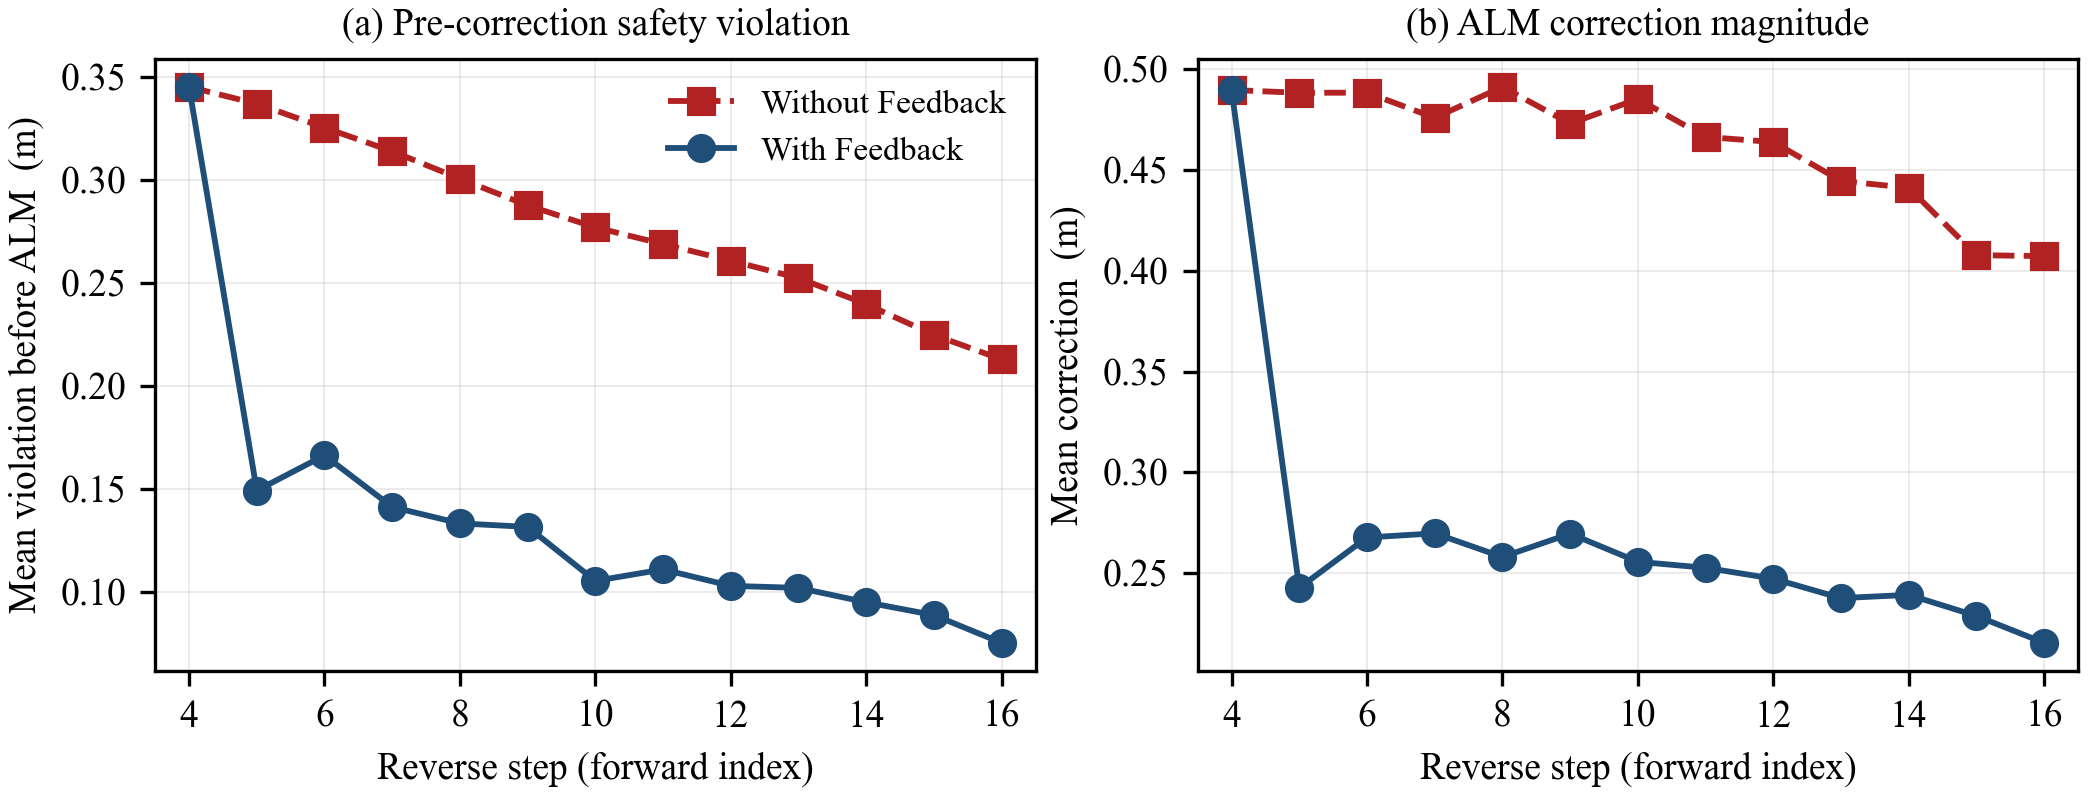
\includegraphics[width=\columnwidth]{fig04_feedback.png}
\caption{Effect of historical safety feedback on the denoising process: (a) mean safety violation before ALM correction; (b) mean ALM correction magnitude.}
\label{fig:feedback}
\end{figure}


% ---------- 源稿 [4.3.2] 段 2 ----------
In the paired statistics over forwards 5--16, enabling the historical feedback
reduces the mean safety violation before ALM correction from 0.2749~m to
0.1167~m (about 57.5\%), and the mean correction magnitude from 0.4609~m to
0.2488~m (about 46.0\%). Both paired tests reach significance (Wilcoxon test,
$p<0.001$). Neither group exhibits any collision in the end, so the effect of
the feedback is mainly to improve how well the intermediate predictions satisfy
the safety constraint and to reduce the correction subsequently required from
the ALM.

\subsection{ALM Iteration Budget Analysis}

\begin{figure}[!htb]
\centering
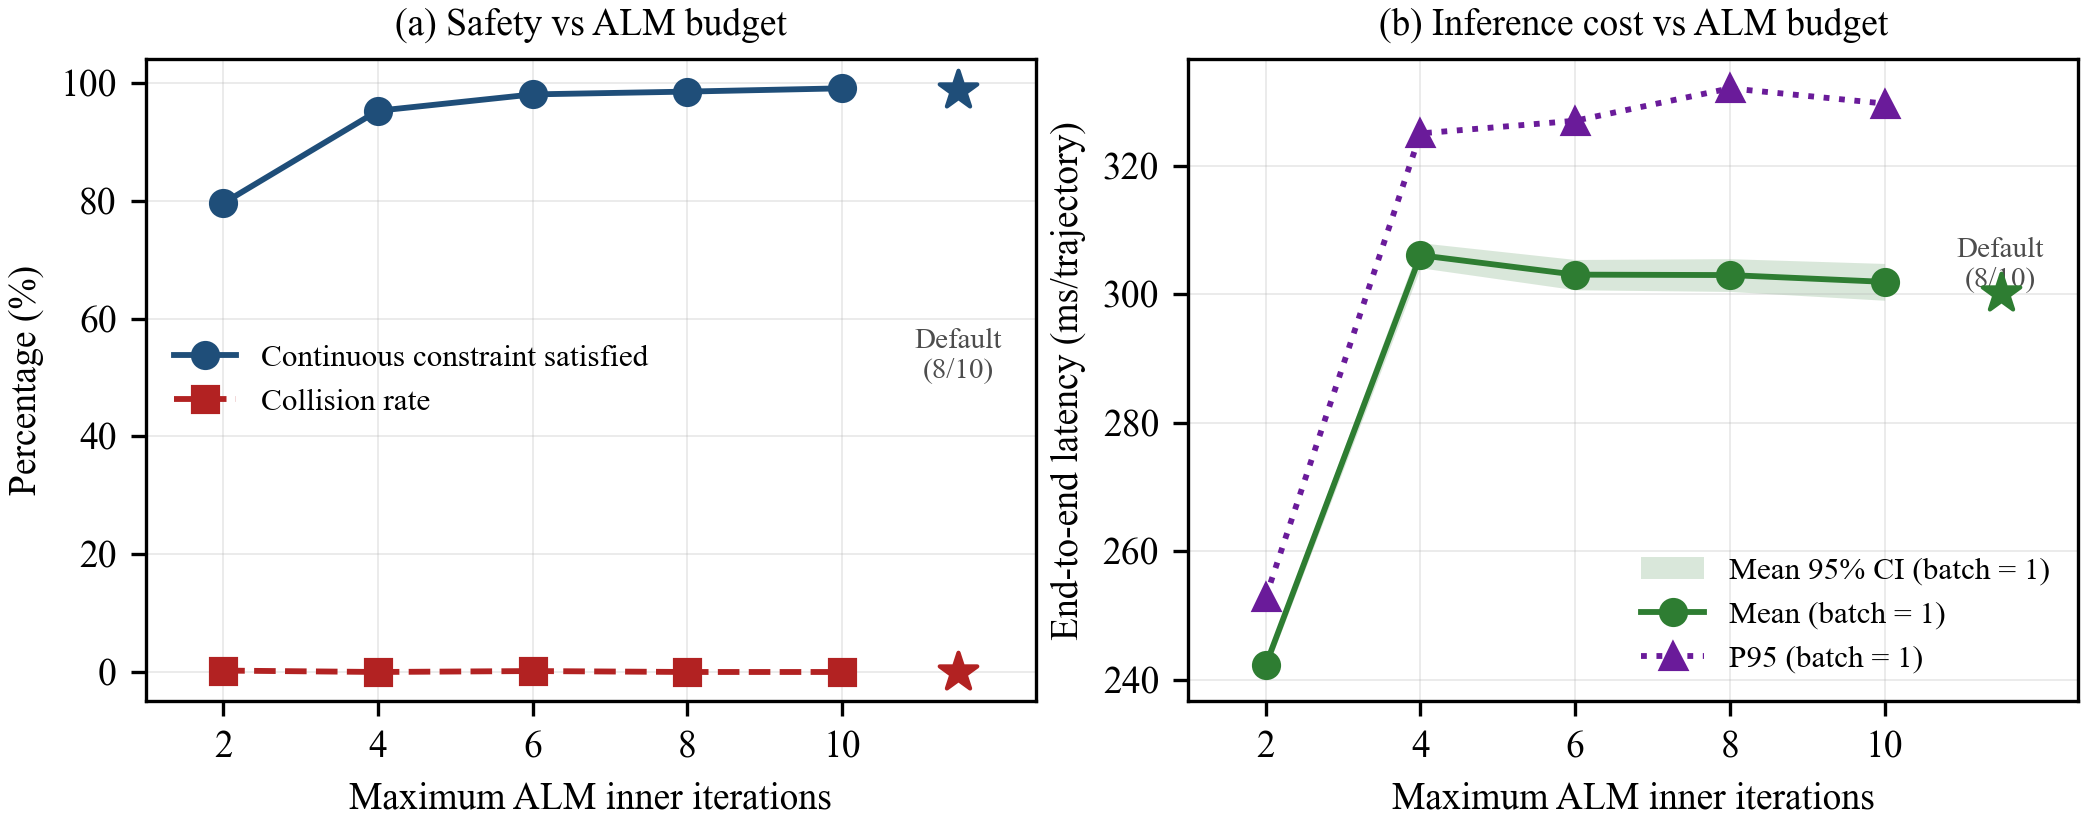
\includegraphics[width=\columnwidth]{fig05_alm_budget.png}
\caption{ALM iteration budget analysis: (a) continuous-constraint satisfaction and collision rate; (b) end-to-end inference cost. The default configuration is marked by a star.}
\label{fig:alm-budget}
\end{figure}


\begin{figure*}[!t]
\centering
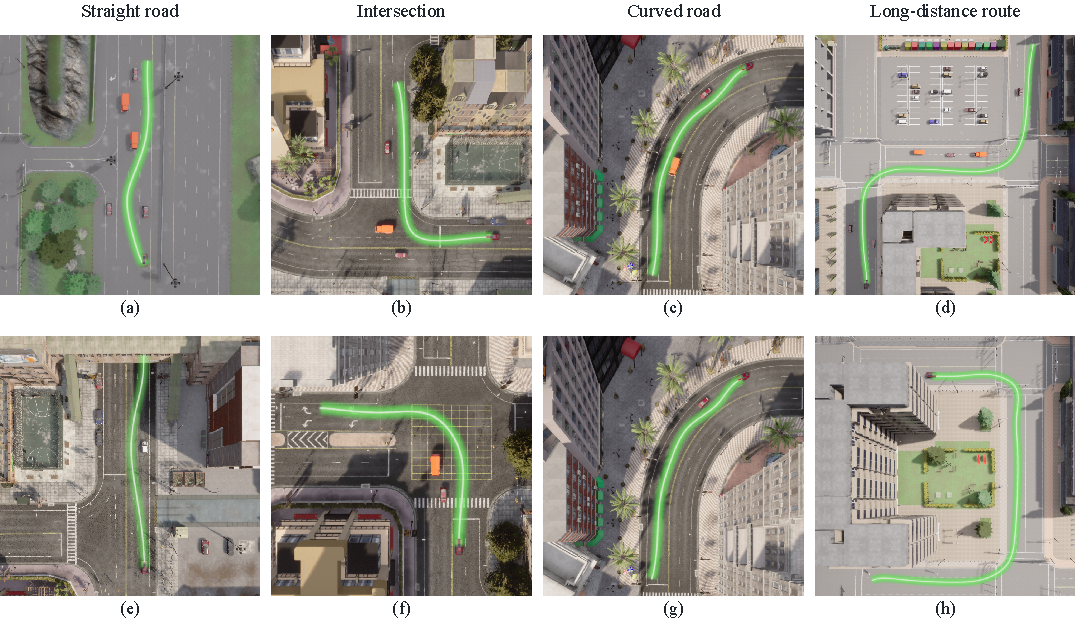
\includegraphics[width=0.82\textwidth]{fig06_carla.pdf}
\caption{Trajectory generation in CARLA road scenes. Columns show straight roads, intersections, curved roads and long-distance routes; the two rows show separate examples. Green bands indicate the drivable range and highlighted centerlines show the generated trajectories.}
\label{fig:carla}
\end{figure*}


% ---------- 源稿 [4.4] 段 1 ----------
Figure~\ref{fig:alm-budget} visualizes the safety--budget relation and inference cost. To assess the influence of the maximum number of ALM inner iterations on safety,
an accelerated inference configuration is used: the model weights, the DDIM step
count, the convex-region sharing scheme and the other optimization parameters are
fixed, and only the maximum ALM iteration count is varied. I2--I10 set the
iteration limit of every ALM call to 2, 4, 6, 8 and 10, respectively, whereas
Default keeps the original strategy of at most 8 iterations for the first call
and at most 10 for the subsequent ones. Iteration stops early under the original
condition once the constraint tolerance is met.

\begin{table}[!t]
\caption{Safety and Trajectory Quality under Different ALM Iteration Budgets}
\label{tab:budget}
\centering
\scriptsize
\setlength{\tabcolsep}{2.5pt}
\begin{tabular}{lccccccc}
\hline
 & Cont.\ feas. & & Clear. & Detour & NRMSE & Max curv. & Mean sq. \\
Config. & (\%) $\uparrow$ & Coll. & (m) $\uparrow$ & ratio $\downarrow$ &
(\%) $\downarrow$ & (1/m) $\downarrow$ & curv. (1/m$^2$) $\downarrow$ \\
\hline
I2  & 79.60 & 3/1260 & 3.221 & 1.3139 & 8.576 & 1.0349 & 0.02087 \\
I4  & 95.32 & 0/1260 & 3.315 & 1.3209 & 8.642 & 1.0499 & 0.02068 \\
I6  & 98.10 & 2/1260 & 3.329 & 1.3216 & 8.659 & 1.0471 & 0.02065 \\
I8  & 98.57 & 0/1260 & 3.321 & 1.3211 & 8.668 & 1.0406 & 0.02057 \\
I10 & 99.13 & 0/1260 & 3.318 & 1.3212 & 8.668 & 1.0436 & 0.02058 \\
\textbf{Default} & \textbf{98.81} & \textbf{0/1260} &
\textbf{3.319} & \textbf{1.3209} & \textbf{8.668} & \textbf{1.0397} &
\textbf{0.02055} \\
\hline
\end{tabular}
\end{table}

% ---------- 源稿 [4.4] 段 2 ----------
Raising the budget from 2 to 4 iterations increases the continuous-constraint
satisfaction rate from 79.60\% to 95.32\%, and 8 iterations reach 98.57\%.
Raising it further to 10 iterations improves the rate by only 0.56 percentage
points, which shows that the return of the iterations gradually saturates.
Paired bootstrap results show that I2 and I4 lie 19.21 and 3.49 percentage
points below Default, with 95\% confidence intervals of
$[-22.78,-15.79]$ and $[-5.48,-1.98]$ percentage points; the intervals of the
differences between I6/I8 and Default contain zero, so the present data do not
establish a difference for the two configurations.

% ---------- 源稿 [4.4] 段 3 ----------
The detour ratio, the NRMSE and the curvature vary little across budgets, which
indicates that the iteration budget mainly affects the degree to which the
continuous constraint is satisfied. The number of collisions does not change
monotonically with the budget, so the budgets cannot be ranked on the basis of a
few discrete collision events alone. Taken together, an overly small iteration
budget markedly degrades the constraint satisfaction rate, whereas a further
increase of the budget brings limited benefit; under the present experimental
setting the current default strategy exhibits the best safety.

\subsection{Trajectory Generation in Real CARLA Road Scenes}
% ---------- 源稿 [4.5] 段 1 ----------
To show how TrajSafe-Diffuser generates trajectories in real road environments,
four scene types, namely straight road segments, intersections, curved road
segments and long-distance routes, are selected in CARLA (Fig.~\ref{fig:carla}); the road and obstacle information is
converted into a two-dimensional occupancy grid and the corresponding B-spline
trajectory is generated. In the planning results, the green translucent band
marks the drivable range of the vehicle and the highlighted centre line marks the
generated trajectory. The proposed method adapts its trajectory to the geometry
of the different road scenes, which complements the quantitative experiments
above.



\end{document}
